\documentclass[1p]{elsarticle_modified}
%\bibliographystyle{elsarticle-num}

%\usepackage[colorlinks]{hyperref}
%\usepackage{abbrmath_seonhwa} %\Abb, \Ascr, \Acal ,\Abf, \Afrak
\usepackage{amsfonts}
\usepackage{amssymb}
\usepackage{amsmath}
\usepackage{amsthm}
\usepackage{scalefnt}
\usepackage{amsbsy}
\usepackage{kotex}
\usepackage{caption}
\usepackage{subfig}
\usepackage{color}
\usepackage{graphicx}
\usepackage{xcolor} %% white, black, red, green, blue, cyan, magenta, yellow
\usepackage{float}
\usepackage{setspace}
\usepackage{hyperref}

\usepackage{tikz}
\usetikzlibrary{arrows}

\usepackage{multirow}
\usepackage{array} % fixed length table
\usepackage{hhline}

%%%%%%%%%%%%%%%%%%%%%
\makeatletter
\renewcommand*\env@matrix[1][\arraystretch]{%
	\edef\arraystretch{#1}%
	\hskip -\arraycolsep
	\let\@ifnextchar\new@ifnextchar
	\array{*\c@MaxMatrixCols c}}
\makeatother %https://tex.stackexchange.com/questions/14071/how-can-i-increase-the-line-spacing-in-a-matrix
%%%%%%%%%%%%%%%

\usepackage[normalem]{ulem}

\newcommand{\msout}[1]{\ifmmode\text{\sout{\ensuremath{#1}}}\else\sout{#1}\fi}
%SOURCE: \msout is \stkout macro in https://tex.stackexchange.com/questions/20609/strikeout-in-math-mode

\newcommand{\cancel}[1]{
	\ifmmode
	{\color{red}\msout{#1}}
	\else
	{\color{red}\sout{#1}}
	\fi
}

\newcommand{\add}[1]{
	{\color{blue}\uwave{#1}}
}

\newcommand{\replace}[2]{
	\ifmmode
	{\color{red}\msout{#1}}{\color{blue}\uwave{#2}}
	\else
	{\color{red}\sout{#1}}{\color{blue}\uwave{#2}}
	\fi
}

\newcommand{\Sol}{\mathcal{S}} %segment
\newcommand{\D}{D} %diagram
\newcommand{\A}{\mathcal{A}} %arc


%%%%%%%%%%%%%%%%%%%%%%%%%%%%%5 test

\def\sl{\operatorname{\textup{SL}}(2,\Cbb)}
\def\psl{\operatorname{\textup{PSL}}(2,\Cbb)}
\def\quan{\mkern 1mu \triangleright \mkern 1mu}

\theoremstyle{definition}
\newtheorem{thm}{Theorem}[section]
\newtheorem{prop}[thm]{Proposition}
\newtheorem{lem}[thm]{Lemma}
\newtheorem{ques}[thm]{Question}
\newtheorem{cor}[thm]{Corollary}
\newtheorem{defn}[thm]{Definition}
\newtheorem{exam}[thm]{Example}
\newtheorem{rmk}[thm]{Remark}
\newtheorem{alg}[thm]{Algorithm}

\newcommand{\I}{\sqrt{-1}}
\begin{document}

%\begin{frontmatter}
%
%\title{Boundary parabolic representations of knots up to 8 crossings}
%
%%% Group authors per affiliation:
%\author{Yunhi Cho} 
%\address{Department of Mathematics, University of Seoul, Seoul, Korea}
%\ead{yhcho@uos.ac.kr}
%
%
%\author{Seonhwa Kim} %\fnref{s_kim}}
%\address{Center for Geometry and Physics, Institute for Basic Science, Pohang, 37673, Korea}
%\ead{ryeona17@ibs.re.kr}
%
%\author{Hyuk Kim}
%\address{Department of Mathematical Sciences, Seoul National University, Seoul 08826, Korea}
%\ead{hyukkim@snu.ac.kr}
%
%\author{Seokbeom Yoon}
%\address{Department of Mathematical Sciences, Seoul National University, Seoul, 08826,  Korea}
%\ead{sbyoon15@snu.ac.kr}
%
%\begin{abstract}
%We find all boundary parabolic representation of knots up to 8 crossings.
%
%\end{abstract}
%\begin{keyword}
%    \MSC[2010] 57M25 
%\end{keyword}
%
%\end{frontmatter}

%\linenumbers
%\tableofcontents
%
\newcommand\colored[1]{\textcolor{white}{\rule[-0.35ex]{0.8em}{1.4ex}}\kern-0.8em\color{red} #1}%
%\newcommand\colored[1]{\textcolor{white}{ #1}\kern-2.17ex	\textcolor{white}{ #1}\kern-1.81ex	\textcolor{white}{ #1}\kern-2.15ex\color{red}#1	}

{\Large $\underline{12n_{0103}~(K12n_{0103})}$}

\setlength{\tabcolsep}{10pt}
\renewcommand{\arraystretch}{1.6}
\vspace{1cm}\begin{tabular}{m{100pt}>{\centering\arraybackslash}m{274pt}}
\multirow{5}{120pt}{
	\centering
	\includegraphics[width=112pt]{../../../GIT/diagram.site/Diagrams/png/2192_12n_0103.png}\\
\ \ \ A knot diagram\footnotemark}&
\allowdisplaybreaks
\textbf{Linearized knot diagam} \\
\cline{2-2}
 &
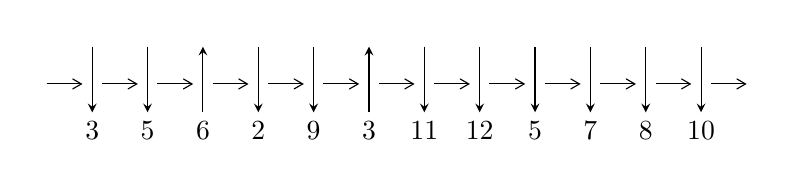
\begin{tikzpicture}[x=20pt, y=17pt]
	% nodes
	\node (C0) at (0, 0) {};
	\node (C1) at (1, 0) {};
	\node (C1U) at (1, +1) {};
	\node (C1D) at (1, -1) {3};

	\node (C2) at (2, 0) {};
	\node (C2U) at (2, +1) {};
	\node (C2D) at (2, -1) {5};

	\node (C3) at (3, 0) {};
	\node (C3U) at (3, +1) {};
	\node (C3D) at (3, -1) {6};

	\node (C4) at (4, 0) {};
	\node (C4U) at (4, +1) {};
	\node (C4D) at (4, -1) {2};

	\node (C5) at (5, 0) {};
	\node (C5U) at (5, +1) {};
	\node (C5D) at (5, -1) {9};

	\node (C6) at (6, 0) {};
	\node (C6U) at (6, +1) {};
	\node (C6D) at (6, -1) {3};

	\node (C7) at (7, 0) {};
	\node (C7U) at (7, +1) {};
	\node (C7D) at (7, -1) {11};

	\node (C8) at (8, 0) {};
	\node (C8U) at (8, +1) {};
	\node (C8D) at (8, -1) {12};

	\node (C9) at (9, 0) {};
	\node (C9U) at (9, +1) {};
	\node (C9D) at (9, -1) {5};

	\node (C10) at (10, 0) {};
	\node (C10U) at (10, +1) {};
	\node (C10D) at (10, -1) {7};

	\node (C11) at (11, 0) {};
	\node (C11U) at (11, +1) {};
	\node (C11D) at (11, -1) {8};

	\node (C12) at (12, 0) {};
	\node (C12U) at (12, +1) {};
	\node (C12D) at (12, -1) {10};
	\node (C13) at (13, 0) {};

	% arrows
	\draw[->,>={angle 60}]
	(C0) edge (C1) (C1) edge (C2) (C2) edge (C3) (C3) edge (C4) (C4) edge (C5) (C5) edge (C6) (C6) edge (C7) (C7) edge (C8) (C8) edge (C9) (C9) edge (C10) (C10) edge (C11) (C11) edge (C12) (C12) edge (C13) ;	\draw[->,>=stealth]
	(C1U) edge (C1D) (C2U) edge (C2D) (C3D) edge (C3U) (C4U) edge (C4D) (C5U) edge (C5D) (C6D) edge (C6U) (C7U) edge (C7D) (C8U) edge (C8D) (C9U) edge (C9D) (C10U) edge (C10D) (C11U) edge (C11D) (C12U) edge (C12D) ;
	\end{tikzpicture} \\
\hhline{~~} \\& 
\textbf{Solving Sequence} \\ \cline{2-2} 
 &
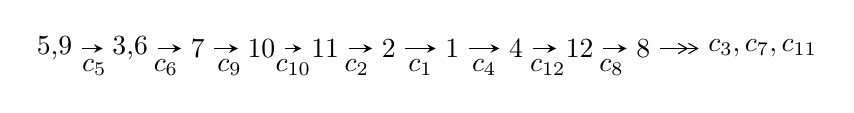
\begin{tikzpicture}[x=23pt, y=7pt]
	% node
	\node (A0) at (-1/8, 0) {5,9};
	\node (A1) at (17/16, 0) {3,6};
	\node (A2) at (17/8, 0) {7};
	\node (A3) at (25/8, 0) {10};
	\node (A4) at (33/8, 0) {11};
	\node (A5) at (41/8, 0) {2};
	\node (A6) at (49/8, 0) {1};
	\node (A7) at (57/8, 0) {4};
	\node (A8) at (65/8, 0) {12};
	\node (A9) at (73/8, 0) {8};
	\node (C1) at (1/2, -1) {$c_{5}$};
	\node (C2) at (13/8, -1) {$c_{6}$};
	\node (C3) at (21/8, -1) {$c_{9}$};
	\node (C4) at (29/8, -1) {$c_{10}$};
	\node (C5) at (37/8, -1) {$c_{2}$};
	\node (C6) at (45/8, -1) {$c_{1}$};
	\node (C7) at (53/8, -1) {$c_{4}$};
	\node (C8) at (61/8, -1) {$c_{12}$};
	\node (C9) at (69/8, -1) {$c_{8}$};
	\node (A10) at (11, 0) {$c_{3},c_{7},c_{11}$};

	% edge
	\draw[->,>=stealth]	
	(A0) edge (A1) (A1) edge (A2) (A2) edge (A3) (A3) edge (A4) (A4) edge (A5) (A5) edge (A6) (A6) edge (A7) (A7) edge (A8) (A8) edge (A9) ;
	\draw[->>,>={angle 60}]	
	(A9) edge (A10);
\end{tikzpicture} \\ 

\end{tabular} \\

\footnotetext{
The image of knot diagram is generated by the software ``\textbf{Draw programme}" developed by Andrew Bartholomew(\url{http://www.layer8.co.uk/maths/draw/index.htm\#Running-draw}), where we modified some parts for our purpose(\url{https://github.com/CATsTAILs/LinksPainter}).
}\phantom \\ \newline 
\centering \textbf{Ideals for irreducible components\footnotemark of $X_{\text{par}}$} 
 
\begin{align*}
I^u_{1}&=\langle 
2.50755\times10^{20} u^{28}-4.57339\times10^{20} u^{27}+\cdots+6.70474\times10^{20} b+2.31276\times10^{20},\\
\phantom{I^u_{1}}&\phantom{= \langle  }4.30865\times10^{20} u^{28}-1.13718\times10^{21} u^{27}+\cdots+6.70474\times10^{20} a+6.48791\times10^{20},\;u^{29}-2 u^{28}+\cdots- u+1\rangle \\
I^u_{2}&=\langle 
b+1,\;u^5+2 u^4+4 u^3+5 u^2+a+4 u+3,\;u^6+u^5+3 u^4+2 u^3+2 u^2+u-1\rangle \\
\\
\end{align*}
\raggedright * 2 irreducible components of $\dim_{\mathbb{C}}=0$, with total 35 representations.\\
\footnotetext{All coefficients of polynomials are rational numbers. But the coefficients are sometimes approximated in decimal forms when there is not enough margin.}
\newpage
\renewcommand{\arraystretch}{1}
\centering \section*{I. $I^u_{1}= \langle 2.51\times10^{20} u^{28}-4.57\times10^{20} u^{27}+\cdots+6.70\times10^{20} b+2.31\times10^{20},\;4.31\times10^{20} u^{28}-1.14\times10^{21} u^{27}+\cdots+6.70\times10^{20} a+6.49\times10^{20},\;u^{29}-2 u^{28}+\cdots- u+1 \rangle$}
\flushleft \textbf{(i) Arc colorings}\\
\begin{tabular}{m{7pt} m{180pt} m{7pt} m{180pt} }
\flushright $a_{5}=$&$\begin{pmatrix}1\\0\end{pmatrix}$ \\
\flushright $a_{9}=$&$\begin{pmatrix}0\\u\end{pmatrix}$ \\
\flushright $a_{3}=$&$\begin{pmatrix}-0.642627 u^{28}+1.69608 u^{27}+\cdots+4.76582 u-0.967660\\-0.373996 u^{28}+0.682112 u^{27}+\cdots+1.36157 u-0.344944\end{pmatrix}$ \\
\flushright $a_{6}=$&$\begin{pmatrix}1\\u^2\end{pmatrix}$ \\
\flushright $a_{7}=$&$\begin{pmatrix}-0.525413 u^{28}+0.870263 u^{27}+\cdots+1.86350 u+0.104816\\-0.165523 u^{28}+0.372194 u^{27}+\cdots+0.644339 u+0.119793\end{pmatrix}$ \\
\flushright $a_{10}=$&$\begin{pmatrix}- u\\u\end{pmatrix}$ \\
\flushright $a_{11}=$&$\begin{pmatrix}0.00550978 u^{28}-0.113964 u^{27}+\cdots-2.05097 u-0.744280\\-0.0294122 u^{28}+0.103634 u^{27}+\cdots+0.884693 u+0.0789002\end{pmatrix}$ \\
\flushright $a_{2}=$&$\begin{pmatrix}-1.01662 u^{28}+2.37819 u^{27}+\cdots+6.12739 u-1.31260\\-0.373996 u^{28}+0.682112 u^{27}+\cdots+1.36157 u-0.344944\end{pmatrix}$ \\
\flushright $a_{1}=$&$\begin{pmatrix}-0.582562 u^{28}+1.02418 u^{27}+\cdots+2.16299 u+0.0440466\\0.0571491 u^{28}-0.153913 u^{27}+\cdots-0.299489 u+0.0607697\end{pmatrix}$ \\
\flushright $a_{4}=$&$\begin{pmatrix}-0.715822 u^{28}+1.86209 u^{27}+\cdots+5.07394 u-0.901780\\-0.390136 u^{28}+0.726358 u^{27}+\cdots+1.45438 u-0.364566\end{pmatrix}$ \\
\flushright $a_{12}=$&$\begin{pmatrix}-0.690936 u^{28}+1.24246 u^{27}+\cdots+2.50784 u+0.224610\\0.165523 u^{28}-0.372194 u^{27}+\cdots-0.644339 u-0.119793\end{pmatrix}$ \\
\flushright $a_{8}=$&$\begin{pmatrix}0.0239024 u^{28}+0.0103299 u^{27}+\cdots+1.16628 u+0.665380\\-0.0294122 u^{28}+0.103634 u^{27}+\cdots+0.884693 u+0.0789002\end{pmatrix}$\\&\end{tabular}
\flushleft \textbf{(ii) Obstruction class $= -1$}\\~\\
\flushleft \textbf{(iii) Cusp Shapes $= \frac{478078822365653903278}{134094852819026608583} u^{28}-\frac{5561400214755760811553}{670474264095133042915} u^{27}+\cdots-\frac{2275460989738397018314}{134094852819026608583} u-\frac{5831311641101896181097}{670474264095133042915}$}\\~\\
\newpage\renewcommand{\arraystretch}{1}
\flushleft \textbf{(iv) u-Polynomials at the component}\newline \\
\begin{tabular}{m{50pt}|m{274pt}}
Crossings & \hspace{64pt}u-Polynomials at each crossing \\
\hline $$\begin{aligned}c_{1}\end{aligned}$$&$\begin{aligned}
&u^{29}+39 u^{28}+\cdots+2258 u+1
\end{aligned}$\\
\hline $$\begin{aligned}c_{2},c_{4}\end{aligned}$$&$\begin{aligned}
&u^{29}-7 u^{28}+\cdots-54 u+1
\end{aligned}$\\
\hline $$\begin{aligned}c_{3},c_{6}\end{aligned}$$&$\begin{aligned}
&u^{29}+5 u^{28}+\cdots+384 u+64
\end{aligned}$\\
\hline $$\begin{aligned}c_{5},c_{9}\end{aligned}$$&$\begin{aligned}
&u^{29}+2 u^{28}+\cdots- u-1
\end{aligned}$\\
\hline $$\begin{aligned}c_{7},c_{8},c_{10}\\c_{11}\end{aligned}$$&$\begin{aligned}
&u^{29}+2 u^{28}+\cdots+5 u+1
\end{aligned}$\\
\hline $$\begin{aligned}c_{12}\end{aligned}$$&$\begin{aligned}
&u^{29}-12 u^{28}+\cdots+3529 u+937
\end{aligned}$\\
\hline
\end{tabular}\\~\\
\newpage\renewcommand{\arraystretch}{1}
\flushleft \textbf{(v) Riley Polynomials at the component}\newline \\
\begin{tabular}{m{50pt}|m{274pt}}
Crossings & \hspace{64pt}Riley Polynomials at each crossing \\
\hline $$\begin{aligned}c_{1}\end{aligned}$$&$\begin{aligned}
&y^{29}-91 y^{28}+\cdots+4903026 y-1
\end{aligned}$\\
\hline $$\begin{aligned}c_{2},c_{4}\end{aligned}$$&$\begin{aligned}
&y^{29}-39 y^{28}+\cdots+2258 y-1
\end{aligned}$\\
\hline $$\begin{aligned}c_{3},c_{6}\end{aligned}$$&$\begin{aligned}
&y^{29}+39 y^{28}+\cdots+212992 y-4096
\end{aligned}$\\
\hline $$\begin{aligned}c_{5},c_{9}\end{aligned}$$&$\begin{aligned}
&y^{29}+30 y^{27}+\cdots+13 y-1
\end{aligned}$\\
\hline $$\begin{aligned}c_{7},c_{8},c_{10}\\c_{11}\end{aligned}$$&$\begin{aligned}
&y^{29}-36 y^{28}+\cdots+13 y-1
\end{aligned}$\\
\hline $$\begin{aligned}c_{12}\end{aligned}$$&$\begin{aligned}
&y^{29}-36 y^{28}+\cdots+62137329 y-877969
\end{aligned}$\\
\hline
\end{tabular}\\~\\
\newpage\flushleft \textbf{(vi) Complex Volumes and Cusp Shapes}
$$\begin{array}{c|c|c}  
\text{Solutions to }I^u_{1}& \I (\text{vol} + \sqrt{-1}CS) & \text{Cusp shape}\\
 \hline 
\begin{aligned}
u &= \phantom{-}0.867238 + 0.470147 I \\
a &= \phantom{-}0.237339 + 1.389930 I \\
b &= -0.92240 - 1.35617 I\end{aligned}
 & -12.12860 - 4.62991 I & -15.7252 + 5.0837 I \\ \hline\begin{aligned}
u &= \phantom{-}0.867238 - 0.470147 I \\
a &= \phantom{-}0.237339 - 1.389930 I \\
b &= -0.92240 + 1.35617 I\end{aligned}
 & -12.12860 + 4.62991 I & -15.7252 - 5.0837 I \\ \hline\begin{aligned}
u &= -0.915025\phantom{ +0.000000I} \\
a &= \phantom{-}0.602737\phantom{ +0.000000I} \\
b &= -2.04399\phantom{ +0.000000I}\end{aligned}
 & -14.6155\phantom{ +0.000000I} & -18.8040\phantom{ +0.000000I} \\ \hline\begin{aligned}
u &= \phantom{-}0.160840 + 1.087590 I \\
a &= \phantom{-}0.0855322 + 0.1114450 I \\
b &= \phantom{-}0.493211 - 0.128104 I\end{aligned}
 & \phantom{-}2.18324 - 1.77578 I & -1.23792 + 3.54893 I \\ \hline\begin{aligned}
u &= \phantom{-}0.160840 - 1.087590 I \\
a &= \phantom{-}0.0855322 - 0.1114450 I \\
b &= \phantom{-}0.493211 + 0.128104 I\end{aligned}
 & \phantom{-}2.18324 + 1.77578 I & -1.23792 - 3.54893 I \\ \hline\begin{aligned}
u &= -0.766809 + 0.460777 I \\
a &= \phantom{-}0.217501 - 1.292190 I \\
b &= -0.793934 + 1.006770 I\end{aligned}
 & -3.36571 + 3.55459 I & -14.7590 - 7.4317 I \\ \hline\begin{aligned}
u &= -0.766809 - 0.460777 I \\
a &= \phantom{-}0.217501 + 1.292190 I \\
b &= -0.793934 - 1.006770 I\end{aligned}
 & -3.36571 - 3.55459 I & -14.7590 + 7.4317 I \\ \hline\begin{aligned}
u &= \phantom{-}0.807312\phantom{ +0.000000I} \\
a &= \phantom{-}0.103435\phantom{ +0.000000I} \\
b &= -1.67794\phantom{ +0.000000I}\end{aligned}
 & -5.54567\phantom{ +0.000000I} & -19.0490\phantom{ +0.000000I} \\ \hline\begin{aligned}
u &= -0.452011 + 1.154640 I \\
a &= -0.089699 - 0.245433 I \\
b &= \phantom{-}0.631471 + 0.354822 I\end{aligned}
 & -4.66125 + 4.01059 I & -6.69076 - 1.05481 I \\ \hline\begin{aligned}
u &= -0.452011 - 1.154640 I \\
a &= -0.089699 + 0.245433 I \\
b &= \phantom{-}0.631471 - 0.354822 I\end{aligned}
 & -4.66125 - 4.01059 I & -6.69076 + 1.05481 I\\
 \hline 
 \end{array}$$\newpage$$\begin{array}{c|c|c}  
\text{Solutions to }I^u_{1}& \I (\text{vol} + \sqrt{-1}CS) & \text{Cusp shape}\\
 \hline 
\begin{aligned}
u &= \phantom{-}0.580536 + 0.452475 I \\
a &= \phantom{-}0.450270 + 1.338160 I \\
b &= -0.597116 - 0.490346 I\end{aligned}
 & -0.77928 - 1.44092 I & -6.71227 + 4.83159 I \\ \hline\begin{aligned}
u &= \phantom{-}0.580536 - 0.452475 I \\
a &= \phantom{-}0.450270 - 1.338160 I \\
b &= -0.597116 + 0.490346 I\end{aligned}
 & -0.77928 + 1.44092 I & -6.71227 - 4.83159 I \\ \hline\begin{aligned}
u &= -0.734655\phantom{ +0.000000I} \\
a &= \phantom{-}1.16704\phantom{ +0.000000I} \\
b &= \phantom{-}0.195873\phantom{ +0.000000I}\end{aligned}
 & -7.96223\phantom{ +0.000000I} & -11.3580\phantom{ +0.000000I} \\ \hline\begin{aligned}
u &= \phantom{-}0.317549 + 0.579846 I \\
a &= \phantom{-}3.74066 + 0.93387 I \\
b &= -0.910186 + 0.367717 I\end{aligned}
 & -10.62150 + 0.95783 I & -12.17772 + 5.24325 I \\ \hline\begin{aligned}
u &= \phantom{-}0.317549 - 0.579846 I \\
a &= \phantom{-}3.74066 - 0.93387 I \\
b &= -0.910186 - 0.367717 I\end{aligned}
 & -10.62150 - 0.95783 I & -12.17772 - 5.24325 I \\ \hline\begin{aligned}
u &= -0.355366 + 0.430210 I \\
a &= \phantom{-}2.58524 - 2.38862 I \\
b &= -0.804622 - 0.092789 I\end{aligned}
 & -2.40653 - 0.39885 I & -18.5948 - 3.1258 I \\ \hline\begin{aligned}
u &= -0.355366 - 0.430210 I \\
a &= \phantom{-}2.58524 + 2.38862 I \\
b &= -0.804622 + 0.092789 I\end{aligned}
 & -2.40653 + 0.39885 I & -18.5948 + 3.1258 I \\ \hline\begin{aligned}
u &= -0.465770\phantom{ +0.000000I} \\
a &= -2.93524\phantom{ +0.000000I} \\
b &= -1.09023\phantom{ +0.000000I}\end{aligned}
 & -2.20812\phantom{ +0.000000I} & \phantom{-}4.71460\phantom{ +0.000000I} \\ \hline\begin{aligned}
u &= \phantom{-}1.12576 + 1.06472 I \\
a &= -0.564004 - 1.170310 I \\
b &= \phantom{-}1.78727 + 0.43721 I\end{aligned}
 & \phantom{-}18.7699 - 11.3822 I & -14.5597 + 4.9176 I \\ \hline\begin{aligned}
u &= \phantom{-}1.12576 - 1.06472 I \\
a &= -0.564004 + 1.170310 I \\
b &= \phantom{-}1.78727 - 0.43721 I\end{aligned}
 & \phantom{-}18.7699 + 11.3822 I & -14.5597 - 4.9176 I\\
 \hline 
 \end{array}$$\newpage$$\begin{array}{c|c|c}  
\text{Solutions to }I^u_{1}& \I (\text{vol} + \sqrt{-1}CS) & \text{Cusp shape}\\
 \hline 
\begin{aligned}
u &= -1.14151 + 1.07839 I \\
a &= -0.559145 + 1.007550 I \\
b &= \phantom{-}1.72676 - 0.31572 I\end{aligned}
 & -11.7546 + 8.6101 I & -13.1323 - 5.7611 I \\ \hline\begin{aligned}
u &= -1.14151 - 1.07839 I \\
a &= -0.559145 - 1.007550 I \\
b &= \phantom{-}1.72676 + 0.31572 I\end{aligned}
 & -11.7546 - 8.6101 I & -13.1323 + 5.7611 I \\ \hline\begin{aligned}
u &= \phantom{-}1.10890 + 1.13111 I \\
a &= -0.839564 - 0.595930 I \\
b &= \phantom{-}1.78058 - 0.11270 I\end{aligned}
 & \phantom{-}18.9482 + 3.1990 I & -14.9528 - 0.8134 I \\ \hline\begin{aligned}
u &= \phantom{-}1.10890 - 1.13111 I \\
a &= -0.839564 + 0.595930 I \\
b &= \phantom{-}1.78058 + 0.11270 I\end{aligned}
 & \phantom{-}18.9482 - 3.1990 I & -14.9528 + 0.8134 I \\ \hline\begin{aligned}
u &= \phantom{-}1.14879 + 1.10311 I \\
a &= -0.592413 - 0.839025 I \\
b &= \phantom{-}1.68896 + 0.17655 I\end{aligned}
 & -8.95243 - 4.17612 I & -10.28879 + 2.37984 I \\ \hline\begin{aligned}
u &= \phantom{-}1.14879 - 1.10311 I \\
a &= -0.592413 + 0.839025 I \\
b &= \phantom{-}1.68896 - 0.17655 I\end{aligned}
 & -8.95243 + 4.17612 I & -10.28879 - 2.37984 I \\ \hline\begin{aligned}
u &= -1.13279 + 1.12536 I \\
a &= -0.701441 + 0.703233 I \\
b &= \phantom{-}1.71752 - 0.02970 I\end{aligned}
 & -11.62970 - 0.31954 I & -13.41116 + 1.33191 I \\ \hline\begin{aligned}
u &= -1.13279 - 1.12536 I \\
a &= -0.701441 - 0.703233 I \\
b &= \phantom{-}1.71752 + 0.02970 I\end{aligned}
 & -11.62970 + 0.31954 I & -13.41116 - 1.33191 I \\ \hline\begin{aligned}
u &= \phantom{-}0.385892\phantom{ +0.000000I} \\
a &= \phantom{-}1.12146\phantom{ +0.000000I} \\
b &= \phantom{-}0.0212520\phantom{ +0.000000I}\end{aligned}
 & -0.763627\phantom{ +0.000000I} & -13.0190\phantom{ +0.000000I}\\
 \hline 
 \end{array}$$\newpage\newpage\renewcommand{\arraystretch}{1}
\centering \section*{II. $I^u_{2}= \langle b+1,\;u^5+2 u^4+4 u^3+5 u^2+a+4 u+3,\;u^6+u^5+3 u^4+2 u^3+2 u^2+u-1 \rangle$}
\flushleft \textbf{(i) Arc colorings}\\
\begin{tabular}{m{7pt} m{180pt} m{7pt} m{180pt} }
\flushright $a_{5}=$&$\begin{pmatrix}1\\0\end{pmatrix}$ \\
\flushright $a_{9}=$&$\begin{pmatrix}0\\u\end{pmatrix}$ \\
\flushright $a_{3}=$&$\begin{pmatrix}- u^5-2 u^4-4 u^3-5 u^2-4 u-3\\-1\end{pmatrix}$ \\
\flushright $a_{6}=$&$\begin{pmatrix}1\\u^2\end{pmatrix}$ \\
\flushright $a_{7}=$&$\begin{pmatrix}1\\u^2\end{pmatrix}$ \\
\flushright $a_{10}=$&$\begin{pmatrix}- u\\u\end{pmatrix}$ \\
\flushright $a_{11}=$&$\begin{pmatrix}- u^3-2 u\\- u^5- u^3+u\end{pmatrix}$ \\
\flushright $a_{2}=$&$\begin{pmatrix}- u^5-2 u^4-4 u^3-5 u^2-4 u-4\\-1\end{pmatrix}$ \\
\flushright $a_{1}=$&$\begin{pmatrix}-1\\0\end{pmatrix}$ \\
\flushright $a_{4}=$&$\begin{pmatrix}- u^5-2 u^4-4 u^3-5 u^2-4 u-3\\-1\end{pmatrix}$ \\
\flushright $a_{12}=$&$\begin{pmatrix}- u^2-1\\u^2\end{pmatrix}$ \\
\flushright $a_{8}=$&$\begin{pmatrix}u^5+2 u^3+u\\- u^5- u^3+u\end{pmatrix}$\\&\end{tabular}
\flushleft \textbf{(ii) Obstruction class $= 1$}\\~\\
\flushleft \textbf{(iii) Cusp Shapes $= -7 u^5-15 u^4-29 u^3-33 u^2-28 u-32$}\\~\\
\newpage\renewcommand{\arraystretch}{1}
\flushleft \textbf{(iv) u-Polynomials at the component}\newline \\
\begin{tabular}{m{50pt}|m{274pt}}
Crossings & \hspace{64pt}u-Polynomials at each crossing \\
\hline $$\begin{aligned}c_{1},c_{2}\end{aligned}$$&$\begin{aligned}
&(u-1)^6
\end{aligned}$\\
\hline $$\begin{aligned}c_{3},c_{6}\end{aligned}$$&$\begin{aligned}
&u^6
\end{aligned}$\\
\hline $$\begin{aligned}c_{4}\end{aligned}$$&$\begin{aligned}
&(u+1)^6
\end{aligned}$\\
\hline $$\begin{aligned}c_{5}\end{aligned}$$&$\begin{aligned}
&u^6+u^5+3 u^4+2 u^3+2 u^2+u-1
\end{aligned}$\\
\hline $$\begin{aligned}c_{7},c_{8}\end{aligned}$$&$\begin{aligned}
&u^6- u^5-3 u^4+2 u^3+2 u^2+u-1
\end{aligned}$\\
\hline $$\begin{aligned}c_{9},c_{12}\end{aligned}$$&$\begin{aligned}
&u^6- u^5+3 u^4-2 u^3+2 u^2- u-1
\end{aligned}$\\
\hline $$\begin{aligned}c_{10},c_{11}\end{aligned}$$&$\begin{aligned}
&u^6+u^5-3 u^4-2 u^3+2 u^2- u-1
\end{aligned}$\\
\hline
\end{tabular}\\~\\
\newpage\renewcommand{\arraystretch}{1}
\flushleft \textbf{(v) Riley Polynomials at the component}\newline \\
\begin{tabular}{m{50pt}|m{274pt}}
Crossings & \hspace{64pt}Riley Polynomials at each crossing \\
\hline $$\begin{aligned}c_{1},c_{2},c_{4}\end{aligned}$$&$\begin{aligned}
&(y-1)^6
\end{aligned}$\\
\hline $$\begin{aligned}c_{3},c_{6}\end{aligned}$$&$\begin{aligned}
&y^6
\end{aligned}$\\
\hline $$\begin{aligned}c_{5},c_{9},c_{12}\end{aligned}$$&$\begin{aligned}
&y^6+5 y^5+9 y^4+4 y^3-6 y^2-5 y+1
\end{aligned}$\\
\hline $$\begin{aligned}c_{7},c_{8},c_{10}\\c_{11}\end{aligned}$$&$\begin{aligned}
&y^6-7 y^5+17 y^4-16 y^3+6 y^2-5 y+1
\end{aligned}$\\
\hline
\end{tabular}\\~\\
\newpage\flushleft \textbf{(vi) Complex Volumes and Cusp Shapes}
$$\begin{array}{c|c|c}  
\text{Solutions to }I^u_{2}& \I (\text{vol} + \sqrt{-1}CS) & \text{Cusp shape}\\
 \hline 
\begin{aligned}
u &= -0.873214\phantom{ +0.000000I} \\
a &= -1.31147\phantom{ +0.000000I} \\
b &= -1.00000\phantom{ +0.000000I}\end{aligned}
 & -9.30502\phantom{ +0.000000I} & -18.5710\phantom{ +0.000000I} \\ \hline\begin{aligned}
u &= \phantom{-}0.138835 + 1.234450 I \\
a &= \phantom{-}0.631845 + 0.143944 I \\
b &= -1.00000\phantom{ +0.000000I}\end{aligned}
 & \phantom{-}1.31531 - 1.97241 I & -11.10050 + 4.53432 I \\ \hline\begin{aligned}
u &= \phantom{-}0.138835 - 1.234450 I \\
a &= \phantom{-}0.631845 - 0.143944 I \\
b &= -1.00000\phantom{ +0.000000I}\end{aligned}
 & \phantom{-}1.31531 + 1.97241 I & -11.10050 - 4.53432 I \\ \hline\begin{aligned}
u &= -0.408802 + 1.276380 I \\
a &= \phantom{-}0.453123 - 0.323434 I \\
b &= -1.00000\phantom{ +0.000000I}\end{aligned}
 & -5.34051 + 4.59213 I & -13.7303 - 5.9632 I \\ \hline\begin{aligned}
u &= -0.408802 - 1.276380 I \\
a &= \phantom{-}0.453123 + 0.323434 I \\
b &= -1.00000\phantom{ +0.000000I}\end{aligned}
 & -5.34051 - 4.59213 I & -13.7303 + 5.9632 I \\ \hline\begin{aligned}
u &= \phantom{-}0.413150\phantom{ +0.000000I} \\
a &= -5.85846\phantom{ +0.000000I} \\
b &= -1.00000\phantom{ +0.000000I}\end{aligned}
 & -2.38379\phantom{ +0.000000I} & -51.7680\phantom{ +0.000000I}\\
 \hline 
 \end{array}$$\newpage
\newpage\renewcommand{\arraystretch}{1}
\centering \section*{ III. u-Polynomials}
\begin{tabular}{m{50pt}|m{274pt}}
Crossings & \hspace{64pt}u-Polynomials at each crossing \\
\hline $$\begin{aligned}c_{1}\end{aligned}$$&$\begin{aligned}
&((u-1)^6)(u^{29}+39 u^{28}+\cdots+2258 u+1)
\end{aligned}$\\
\hline $$\begin{aligned}c_{2}\end{aligned}$$&$\begin{aligned}
&((u-1)^6)(u^{29}-7 u^{28}+\cdots-54 u+1)
\end{aligned}$\\
\hline $$\begin{aligned}c_{3},c_{6}\end{aligned}$$&$\begin{aligned}
&u^6(u^{29}+5 u^{28}+\cdots+384 u+64)
\end{aligned}$\\
\hline $$\begin{aligned}c_{4}\end{aligned}$$&$\begin{aligned}
&((u+1)^6)(u^{29}-7 u^{28}+\cdots-54 u+1)
\end{aligned}$\\
\hline $$\begin{aligned}c_{5}\end{aligned}$$&$\begin{aligned}
&(u^6+u^5+3 u^4+2 u^3+2 u^2+u-1)(u^{29}+2 u^{28}+\cdots- u-1)
\end{aligned}$\\
\hline $$\begin{aligned}c_{7},c_{8}\end{aligned}$$&$\begin{aligned}
&(u^6- u^5-3 u^4+2 u^3+2 u^2+u-1)(u^{29}+2 u^{28}+\cdots+5 u+1)
\end{aligned}$\\
\hline $$\begin{aligned}c_{9}\end{aligned}$$&$\begin{aligned}
&(u^6- u^5+3 u^4-2 u^3+2 u^2- u-1)(u^{29}+2 u^{28}+\cdots- u-1)
\end{aligned}$\\
\hline $$\begin{aligned}c_{10},c_{11}\end{aligned}$$&$\begin{aligned}
&(u^6+u^5-3 u^4-2 u^3+2 u^2- u-1)(u^{29}+2 u^{28}+\cdots+5 u+1)
\end{aligned}$\\
\hline $$\begin{aligned}c_{12}\end{aligned}$$&$\begin{aligned}
&(u^6- u^5+3 u^4-2 u^3+2 u^2- u-1)(u^{29}-12 u^{28}+\cdots+3529 u+937)
\end{aligned}$\\
\hline
\end{tabular}\newpage\renewcommand{\arraystretch}{1}
\centering \section*{ IV. Riley Polynomials}
\begin{tabular}{m{50pt}|m{274pt}}
Crossings & \hspace{64pt}Riley Polynomials at each crossing \\
\hline $$\begin{aligned}c_{1}\end{aligned}$$&$\begin{aligned}
&((y-1)^6)(y^{29}-91 y^{28}+\cdots+4903026 y-1)
\end{aligned}$\\
\hline $$\begin{aligned}c_{2},c_{4}\end{aligned}$$&$\begin{aligned}
&((y-1)^6)(y^{29}-39 y^{28}+\cdots+2258 y-1)
\end{aligned}$\\
\hline $$\begin{aligned}c_{3},c_{6}\end{aligned}$$&$\begin{aligned}
&y^6(y^{29}+39 y^{28}+\cdots+212992 y-4096)
\end{aligned}$\\
\hline $$\begin{aligned}c_{5},c_{9}\end{aligned}$$&$\begin{aligned}
&(y^6+5 y^5+\cdots-5 y+1)(y^{29}+30 y^{27}+\cdots+13 y-1)
\end{aligned}$\\
\hline $$\begin{aligned}c_{7},c_{8},c_{10}\\c_{11}\end{aligned}$$&$\begin{aligned}
&(y^6-7 y^5+\cdots-5 y+1)(y^{29}-36 y^{28}+\cdots+13 y-1)
\end{aligned}$\\
\hline $$\begin{aligned}c_{12}\end{aligned}$$&$\begin{aligned}
&(y^6+5 y^5+9 y^4+4 y^3-6 y^2-5 y+1)\\
&\cdot(y^{29}-36 y^{28}+\cdots+62137329 y-877969)
\end{aligned}$\\
\hline
\end{tabular}
\vskip 2pc
\end{document}